\documentclass{article}
\usepackage{graphicx} % Required for inserting images
\usepackage{wrapfig}
\usepackage{tikz}
\usetikzlibrary{shapes.geometric, arrows}
\usepackage{caption}
\captionsetup[figure]{labelformat=empty}

\title{Phys 494 Final Design Brief}
\author{Aidan Hill, Terrance Jones, and Madison Niemi}
\date{\today}
\graphicspath{{images/}}

\begin{document}

\maketitle

\begin{figure}[h!]
    \centering
    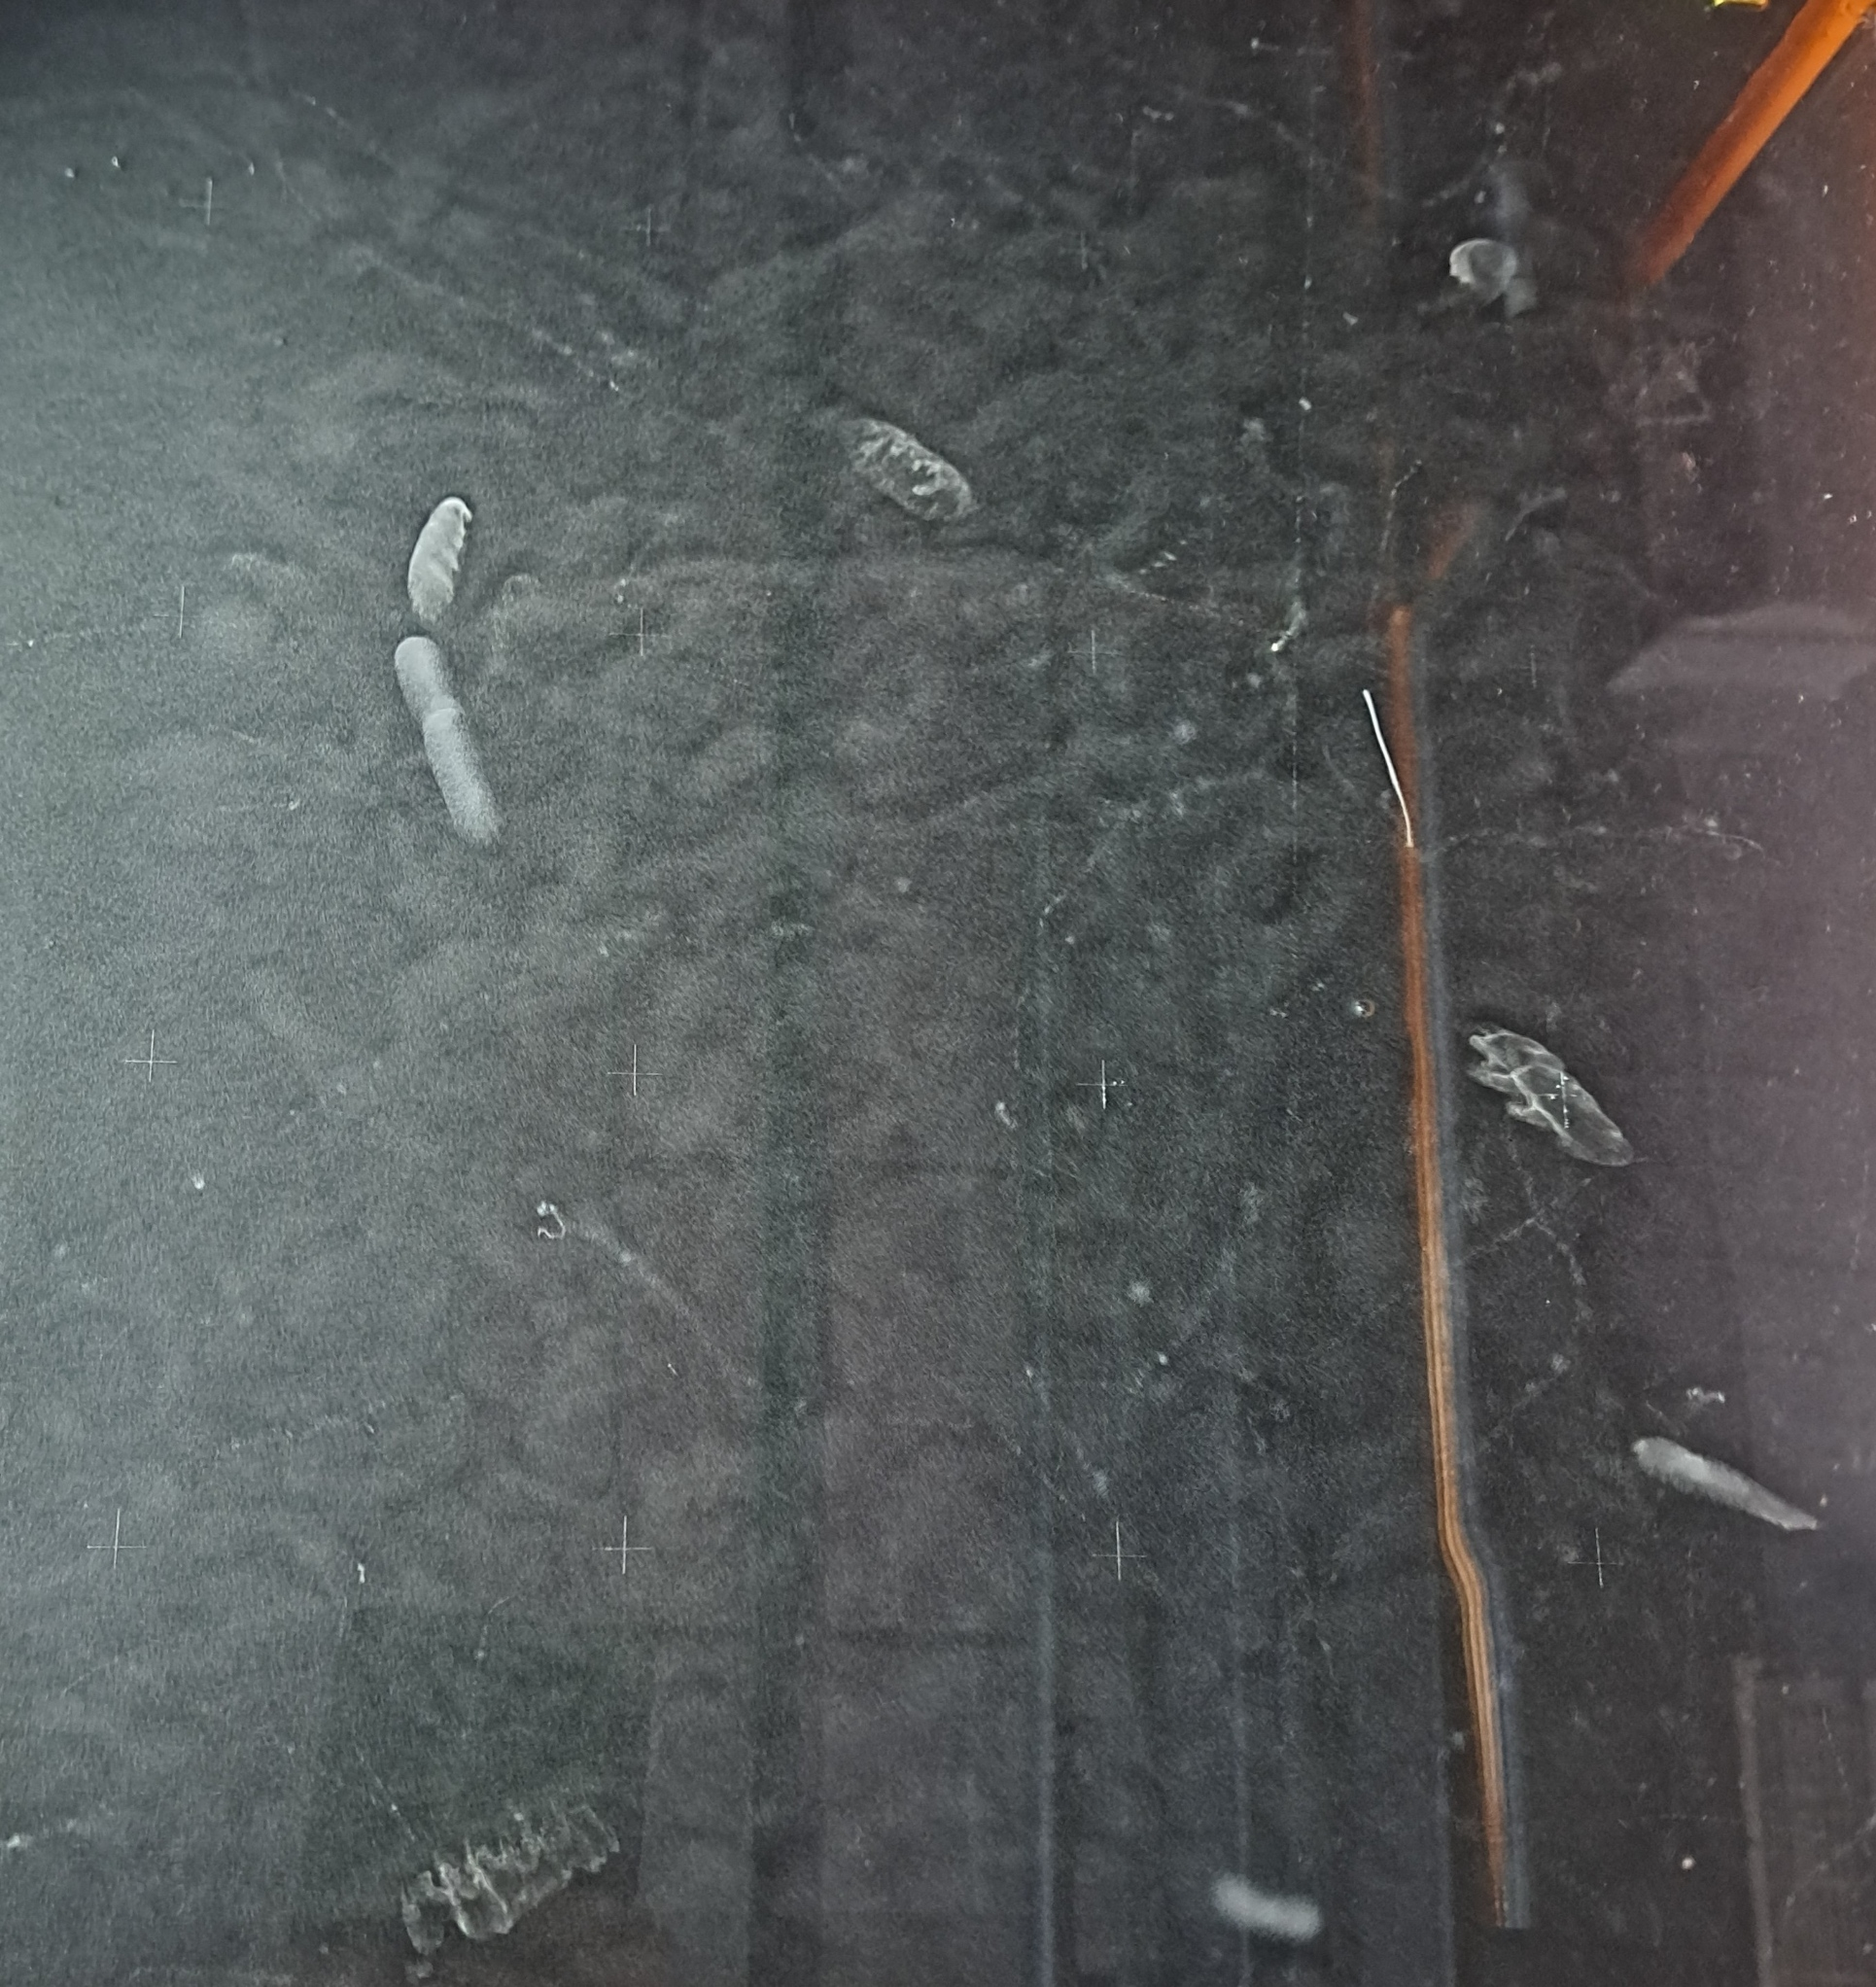
\includegraphics[width=1\linewidth]{10}
    \caption{Image of Dr. Lee's Cloud chamber with charged particle activity.}
\end{figure}

\newpage
\section{Introduction}
Cosmic rays are high-energy particles originating from outer space that constantly bombard the Earth, passing through us undetected every second. These particles, primarily protons and atomic nuclei, travel at nearly the speed of light, originating from supernovae, distant galaxies, and even mysterious cosmic phenomena. Despite their omnipresence, cosmic rays remain largely invisible to the human senses. The Cosmic Rave seeks to bridge this gap by transforming the unseen world of cosmic rays into a fully immersive, interactive experience.
\\
\\  Combining physics and interior architecture, this project translates cosmic ray interactions into a dynamic audiovisual spectacle. Through the use of visible light, dynamic projections, and music, The Cosmic Rave brings the energy and motion of these high-energy particles to life. Visitors will enter a space where they can see, hear, and feel the presence of cosmic rays in a way never before experienced. By blending scientific accuracy with creative storytelling and design, this project fosters curiosity, encourages interdisciplinary exploration, and enhances public engagement with astrophysics. Ultimately, The Cosmic Rave serves as an innovative model for making complex scientific concepts accessible, inspiring wonder, and offering a memorable journey into the unseen forces that shape our universe.

\section{Thesis Statement}
By combining interior design, music design, and physics, The Cosmic Rave renders the intangible existence of cosmic rays into a visceral, experiential reality, demonstrating the power of immersive design to instruct, engage, and motivate.

\section{Investigative Process}
\begin{wrapfigure}{r}{0.35\textwidth}
  \begin{center}
    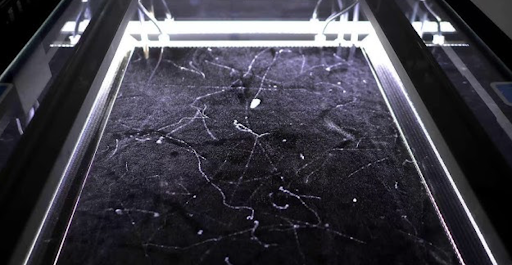
\includegraphics[width=0.3\textwidth]{1}
  \end{center}
  \caption{OpenAI generated image of a cloud chamber.}
\end{wrapfigure}
Grouping our semester into three sections allows for a better understanding of what occurred. Learning, Exploring, and Prototyping. 

\subsection{Learning}
We kicked off the semester with a live demonstration of what a cosmic ray looks like. By looking at a cloud chamber we were able to see  the tracks of subatomic particles as they pass through the chamber, visualizing their paths. The chamber is filled with a supersaturated vapor, and when charged 	
particles pass through, they ionize the vapor, causing tiny droplets to condense along their paths, creating visible tracks (open.ai). This experience kick started our exploration of the cosmics by showing a tangible experience that captures our goal of seeing the unseen. 
\\\\
During the next phase of this course we were asked a few questions: \textit{What is science, what is design, and how can we marry the two for a unique, impactful experience?}

\subsubsection{\textit{What is science:}}
We define science as inquiry through scientific and creative means of communication. We discussed what a measurement is describing as a qualification of attributes that yields some type of information gain. It was important for us to understand the tools used to gather this information. Translation is a factor that we rely on when exploring light. We cannot measure light with our eyes, so we used measurement tools to extend our own sensing capabilities. 

\subsubsection{Design}
Design is the process that measures possibilities through creativity and discovery to make meaningful experiences. We were given a five step process of design: 
\\

\begin{center}
\begin{figure}[h!]
\begin{center}
\tikzstyle{startstop} = [
minimum width=3cm, 
minimum height=.7cm,
text centered]
\begin{tikzpicture}[node distance=1.2cm]


\node (1) [startstop] {\textbf{Intention:} Discovery and Creativity};
\node (2) [startstop, below of=1] {\textbf{Essence:} What is it?};
\node (3) [startstop, below of=2] {\textbf{Context:} Unique constraints and limitations};
\node (4) [startstop, below of=3] {\textbf{Metaphor:} Describe the future 
};
\node (5) [startstop, below of=4] {\textbf{Vocabulary:} Verbs and then Nouns};
\draw (1) -- (2);
\draw (2) -- (3);
\draw (3) -- (4);
\draw (4) -- (5);
\end{tikzpicture}
\end{center}
\caption{\textit{“It's not what we intend, but is what is found meaningful” 
\\ - Matthews 
}}
\end{figure}
\end{center}
The key takeaways were purpose beyond practicality and we must take the essence and transform it. Nijiriguchi (Push down mouth) 

\subsubsection{Lifecycle of Cosmic Rays}
Cosmic rays begin their lives at astrophysical sources such as stars, supernoavae, and black holes. These sources shoot off long lived particles, lifetimes greater than 10$^6$ years, that travel through space. We call these long lived particles made up primarily of protons, atomic nuclei, and neutrinos, primary particles. These particles travel through space, and when they hit the upper atmosphere they react. Protons decay into pions, and pions decay into muons and neutrinos. These muons are charged particles, like an electron with 200 times the mass. These decay showers are called secondary particles\footnote{A paper about muon decay https://www.ucl.ac.uk/~zcapg66/work/Muon.pdf}. This means that when as they descend to Earth we see them in any number of charged particle detectors (something like a cloud chamber, scintillator, or solid state detector). This allows for the detection of secondary comics at the surface of Earth. However, these muons have an average lifetime of 2.2 $\mu s$. This does not allow muons to reach the surface of the Earth from the upper atmosphere, but we still see them. What is happening?
\\\\
To solve this conundrum we must introduce the concept of special relativity. In the most basic sense, special relativity changes the way that space and time are experienced determined by the frame (point of view) of the observer. For instance, in the Earth frame, the muon lives longer than the 2.2 $\mu s$ that it lives in its rest frame. We can express this time as $t = \gamma t'$ with $t'$ being the time in the muon frame. Likewise, in the muon frame, the length contracts by a factor $l' = \frac{l}{\gamma}$. This means that, according to the muon, it does not have to travel as far to reach the surface of the Earth. This is the effect that allows us to see the muon at the Earth's surface. \footnote{Basic reading on the subject can be found here https://openstax.org/books/university-physics-volume-3/pages/5-introduction}
\begin{figure}[h!]
    \centering
    \includegraphics[width=0.5\linewidth]{425}
    \caption{A poster describing the lifecycle of a cosmic ray. Made by Natalie Hugo.}
    \label{fig:enter-label}
\end{figure}


\subsection{Exploring}
We were divided into four groups–each tasked with a different design element: 
\\\\
\begin{wrapfigure}{r}{0.48\textwidth}
  \begin{center}
    \begin{subfigure}
    \begin{center}
        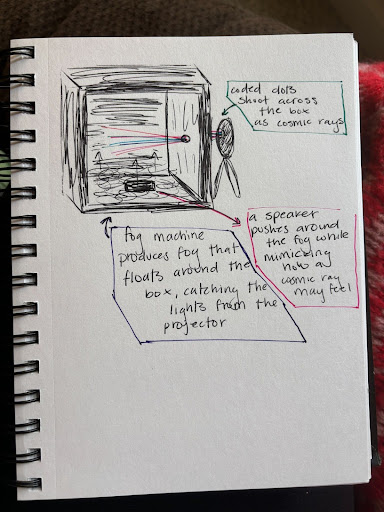
\includegraphics[width=0.4\textwidth]{3}
    \end{center}
    \end{subfigure}
  \begin{subfigure}
  \begin{center}
    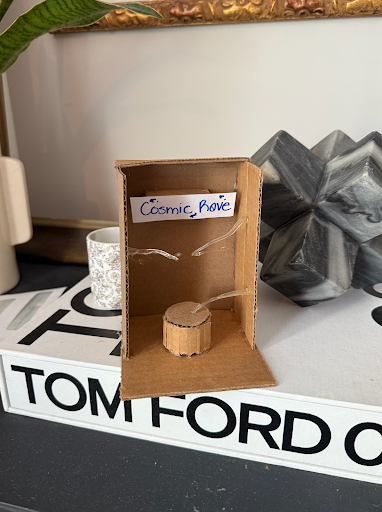
\includegraphics[width=0.4\textwidth]{4}
  \end{center}
  \end{subfigure}
  \end{center}
  \caption{Initial sketch and abstract 3D design by Terrance.}
\end{wrapfigure}
My group was tasked with creating an experience that emphasized the use of a line element. Each member 
was assigned to quickly prototype a concept that highlighted their chosen criteria. We were told our constraints would consist of a 1'x1'x1 cube to display our design and, if possible, would be constructed of scrap materials. Professor Matthews and Dr. Lee would provide any other materials needed to accomplish our design. The main focus of each group's design was to capture the attention of visitors while also providing a clear, visual representation of a cosmic ray. After some brainstorming and sketching out ideas, we decided as a group that we wanted bright lights and music to be the focus of our design. This led to the initial creation of the Cosmic Rave. We were limited to 
using only household materials and given just 30 
minutes to complete our initial prototypes. For my prototype, I used cardboard to represent the room and stage, while 
hot glue strands symbolized the cosmic rays—our interpretation of the light elements in the rave experience. Ultimately, my prototype is the one we decided to base our design off of moving forward. 
\\\\
From here each person was asked to come up with general questions. We placed all these questions, grouped them together on a board and narrowed down which questions we deemed most important when designing our experiences. Our four questions were: 
\begin{wrapfigure}{r}{0.34\textwidth}
  \begin{center}
    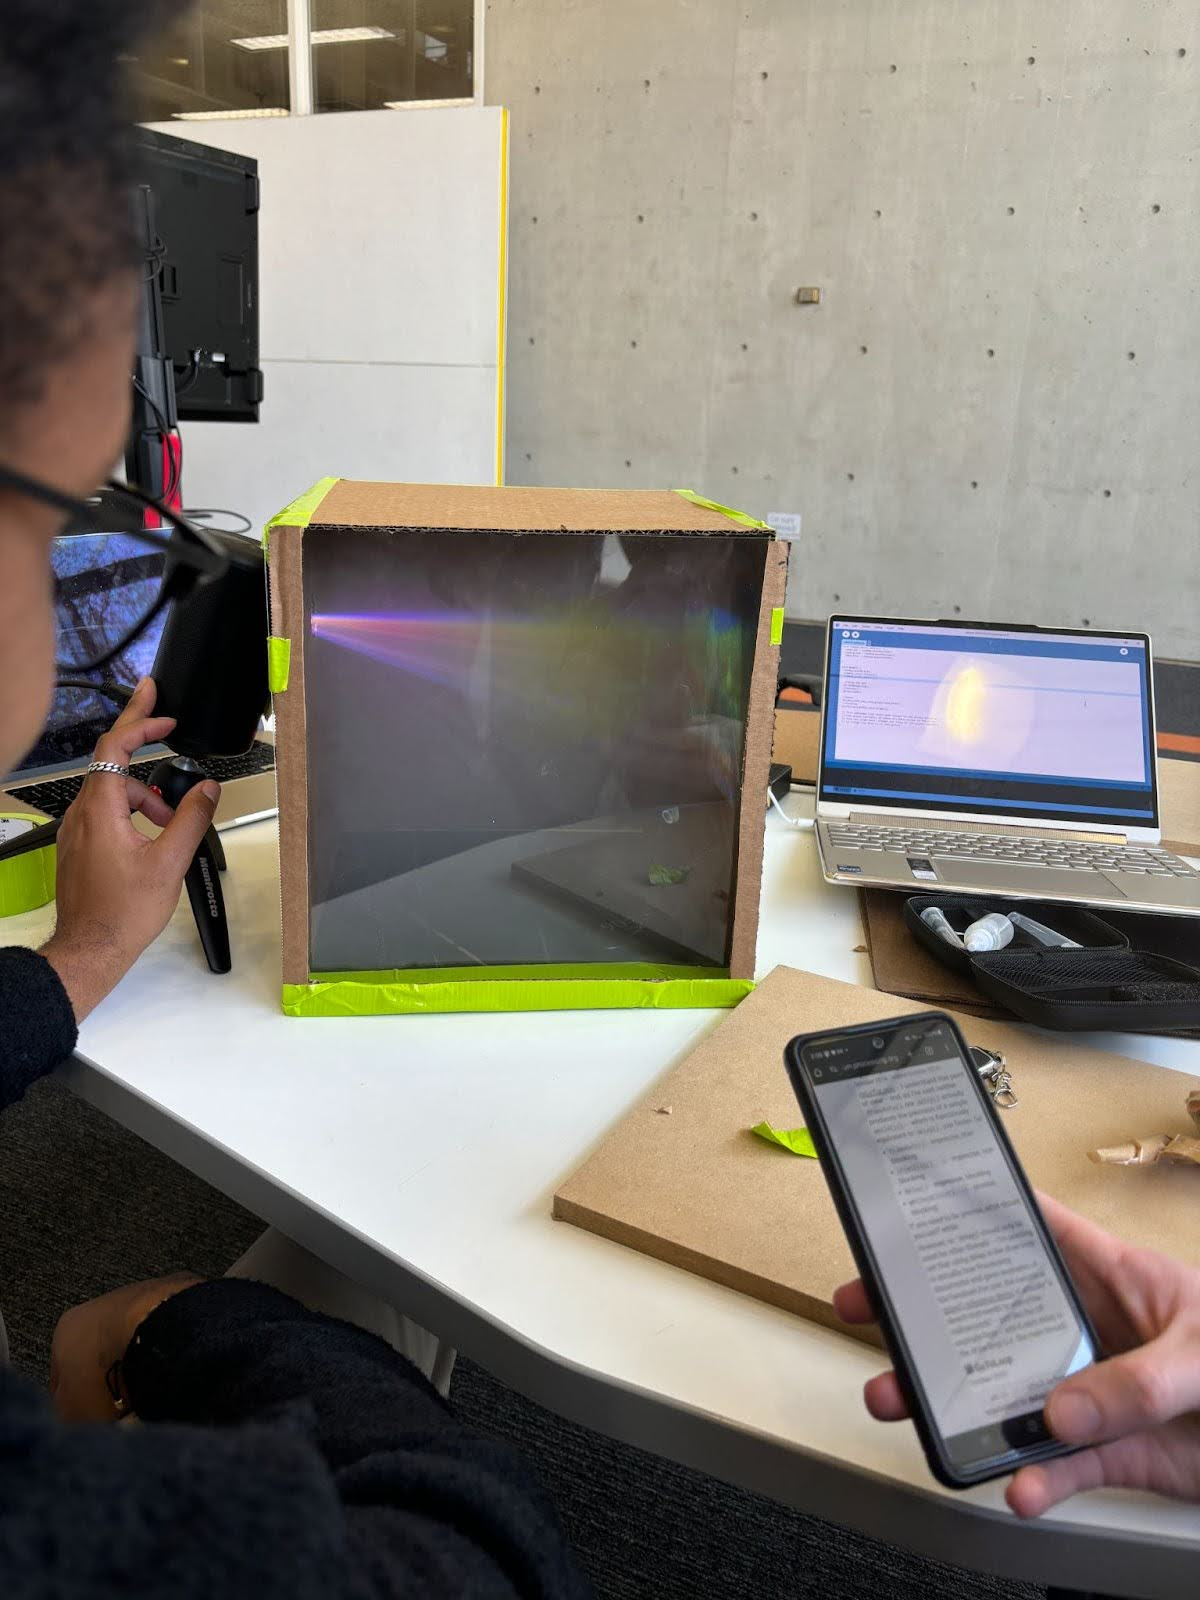
\includegraphics[width=0.3\textwidth]{6}
  \end{center}
  \caption{Initial testing of first prototype.}
\end{wrapfigure}

\begin{enumerate}
    \item Are all of our senses required for perceiving comic rays?
    \item Can sound be translated to reflect the feeling of the cosmic rays around us? 
    \item What would a musical representation of a cosmic ray feel/sound like? 
    \item What scientific materials would be required to measure a cosmic ray?
\end{enumerate}
Now it was time to create something. Originally we planned to 3D print a 1’x1’x1’ box to house our experience, but due to technical difficulties with the 3D print file we were unable to. However, we were able to construct a working prototype out of cardboard that we would use for the majority of the semester. We cut a hole in one wall of the cube so that the projector would have a space to project through. We used a small projector to create lines of light that defused across a fog machine induced membrane. To achieve the fog effect we were hoping for, we cut a small hole in the bottom of one of the walls of the cube and fed the fog machine tube through it. After some iteration and a few presentations, we ended up moving the hole for the fog machine to the top of the cube. We knew we wanted the box to be dark to imitate space and to enhance the effectiveness of the projector, so we began brainstorming how we might achieve that.

\subsubsection{\textit{Programming?}}

A rave is incomplete without a light show, and the light allows a artistic visual representation of cosmic rays. We chose to use light to explore the dimensionality of lines in our box. To implement this we wanted to project light through a medium like lasers at a rave. The goal was to create a sense of lines passing through space, much like cosmic ray showers passing down to Earth from the upper atmosphere. 
\\\\
We began with Aidan coding a basic sketch in a language called processing. This java based language allowed for a visual and auditory output and was recommended by our professor, Dr. Lee. The first sketch was simple. It created a random number of dots in random positions on the screen at set time intervals. This ended up looking like a strobe in the box and lacked a sense of motion that we saw in the cloud chamber at the beginning of the semester. This was presented at the midway point through the semester and we got a little bit of feedback on it. It looked too rigid, the dots needed to be independent, and there needed to be some link to a physical significance.
\\\\
 This led to the second visual iteration\footnote{Contained in the repo https://github.com/ahill117/PHYS494-ARC425}. Here the programming philosophy switched from just a basic sketch to a basic object oriented sketch. The way it works is that a hit object is created corresponding with some random time. The object is selected along an energy curve of cosmic rays (given by Dr. Lee in one of our homeworks). From this value, a color and sound are generated. Other attributes randomly generated at creation are the lifetime and size of hit. The hit is then drawn onto the screen, animated to fade out and slightly fall, and passed through to a projector, which outputs the screen through the foggy box. This creates a visual of motion of lines, similar but not the same as what we saw in the cloud chamber. It also passes the midi output to a 3rd party program to be played along with music. This is further discussed in the below section.

 \subsubsection{\textit{Music?}}
 Likewise a rave is incomplete without music, and sound adds an essential sensory layer that makes an experience both immersive and memorable. Initially, we wanted the music element to be playing through a large speaker that visitors would sit on while viewing the experience. This way they would feel the effect of the music while watching the projected rays. After a few presentations we realized that the music element would be most effective through the use of headphones. For our final two presentations, we had the viewers wear headphones while watching the projections. We hope for the future, full-scale exhibit, that we can migrate back to the bench-speaker idea.
 \\\\
 To elevate the Cosmic Rave, Terrance composed an original piece using sounds commonly associated with space. The audio composition transports the audience through deep subwoofer frequencies and piercing soprano tones—his imaginative rendering of what cosmic rays might sound like if they were audible to the human ear.
 \\\\
To bridge the gap between sound and visuals, each MIDI note from the composition was programmed to trigger corresponding light outputs. The steady rhythm of the piece reflects the constant pulse of cosmic energy, while the randomized notes controlling the lights mirror the chaotic, unpredictable nature of cosmic rays themselves. The notes themselves are selected chromatically and correspond to energy level. They are then passed from processing to a software like Garage Band where they can be outputted with Terrance's composition.



\section{Outcomes}

With the concept finalized, it was time to move into the build phase. The cube was constructed from black scrap wood, secured using screws, glue, and double-sided tape. One side of the box features two openings—one for a fog machine and the other for a projector. These were made in alignment with the measurements of the projector and fog machine. The interior wall opposite the projector is lined with black felt, which helps absorb excess light to reduce visual noise from the projection and further drives home the idea of our cube representing space. Symbolically, the felt also represents materials that could be used to soundproof a full-scale Cosmic Rave installation.
\\\\
\begin{wrapfigure}{r}{0.5\textwidth}
  \begin{center}
  \begin{subfigure}
      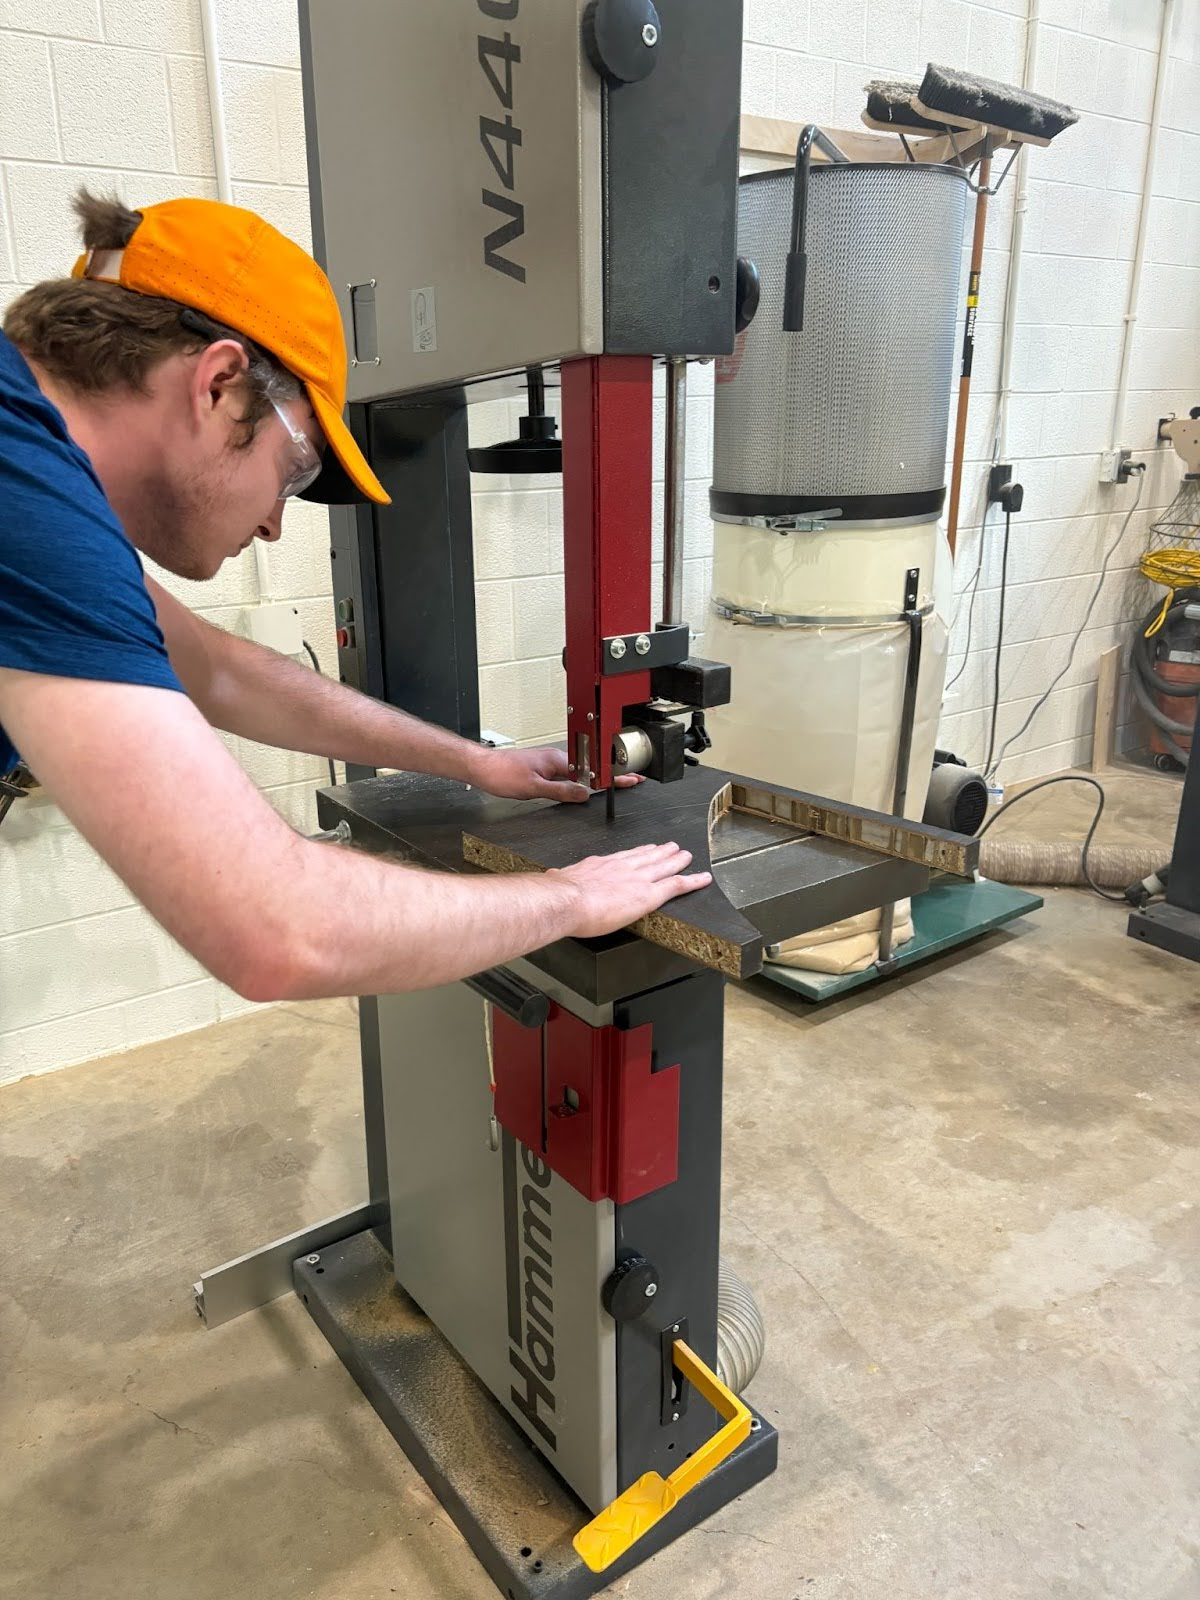
\includegraphics[width=0.23\textwidth]{7}
  \end{subfigure}
  \begin{subfigure}
    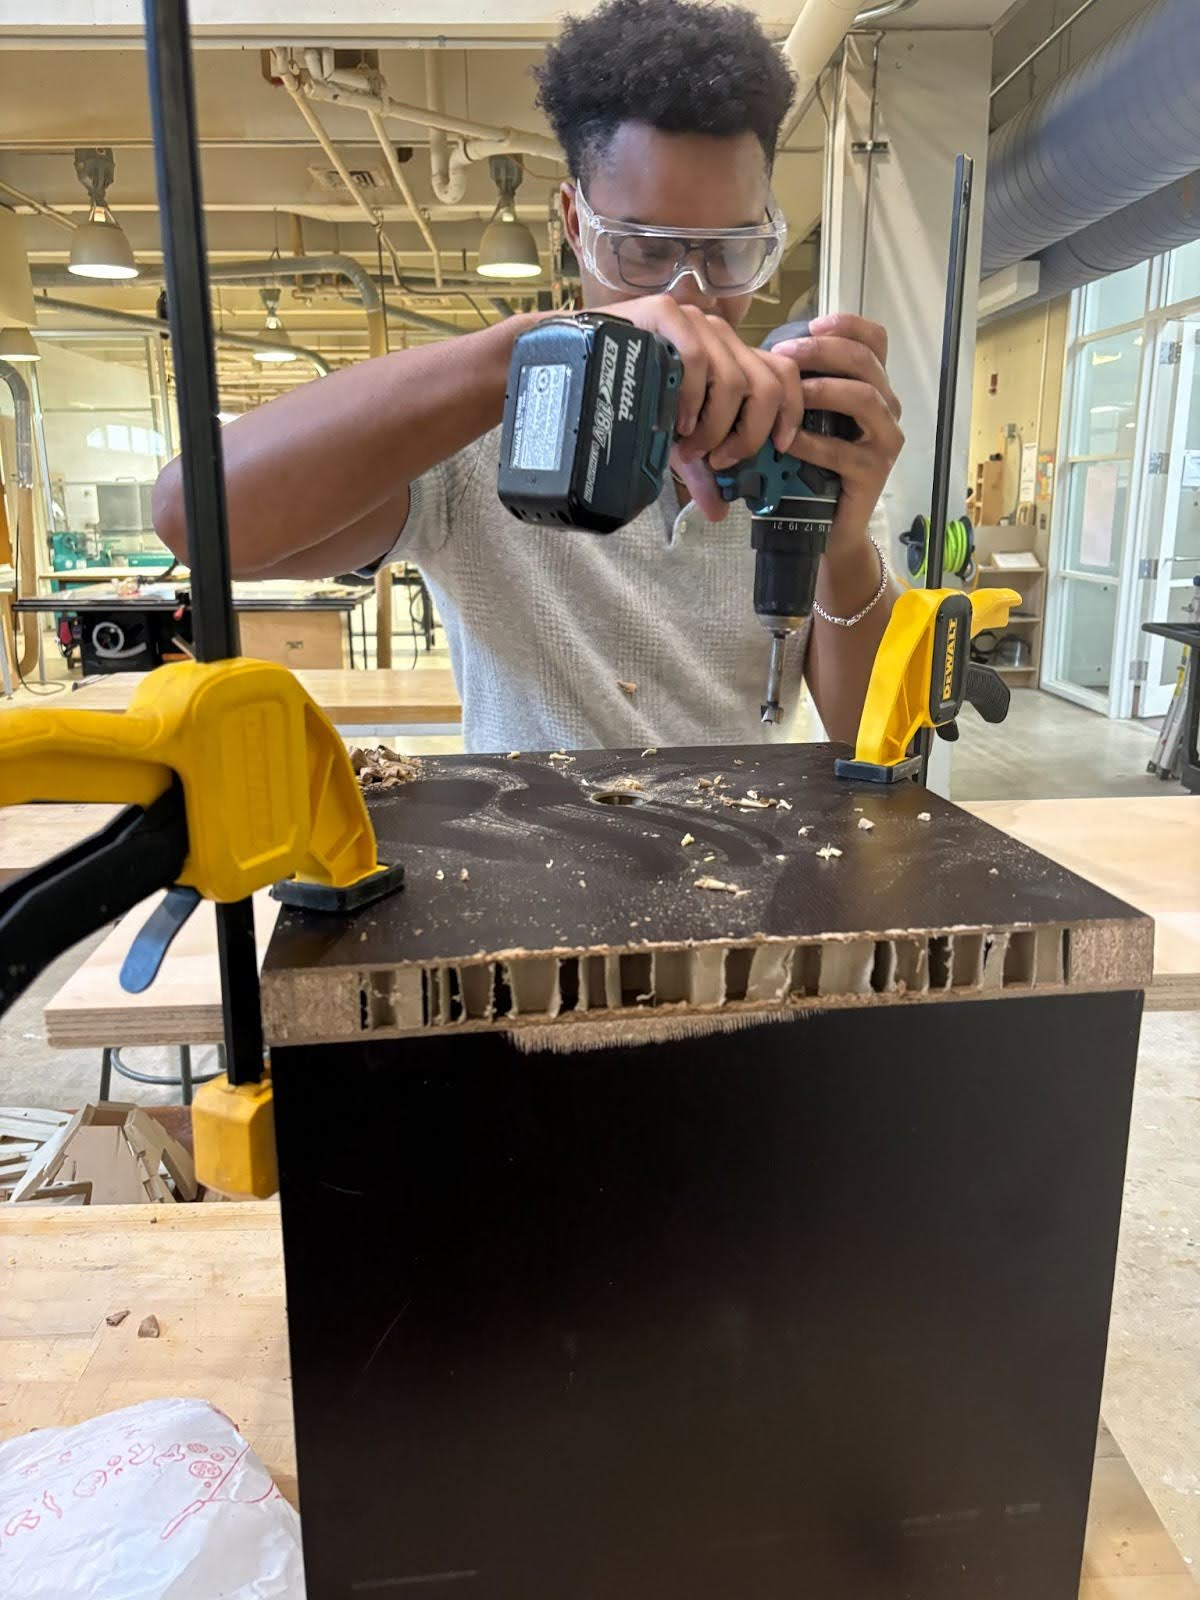
\includegraphics[width=0.23\textwidth]{8}
  \end{subfigure}
  \end{center}
  \caption{Aidan and Terrance working on the final box}
\end{wrapfigure}
The front of the box is made of clear plexiglass, allowing viewers to peer inside and witness the rave in action while keeping the fog contained within the space. Initially, we had considered having the option to switch out the clear plexiglass for different colored sheets of plexiglass to briefly study color theory and how it may add to the experience. After giving it a try, we discovered it only hurt our project due to it making most of our lights near impossible to see. We decided to stick to using only the clear plexiglass, which preserved both the atmosphere and the integrity of the Cosmic Rave.

\subsection{Final Prototype}
\begin{wrapfigure}{r}{0.3\textwidth}
\begin{center}
    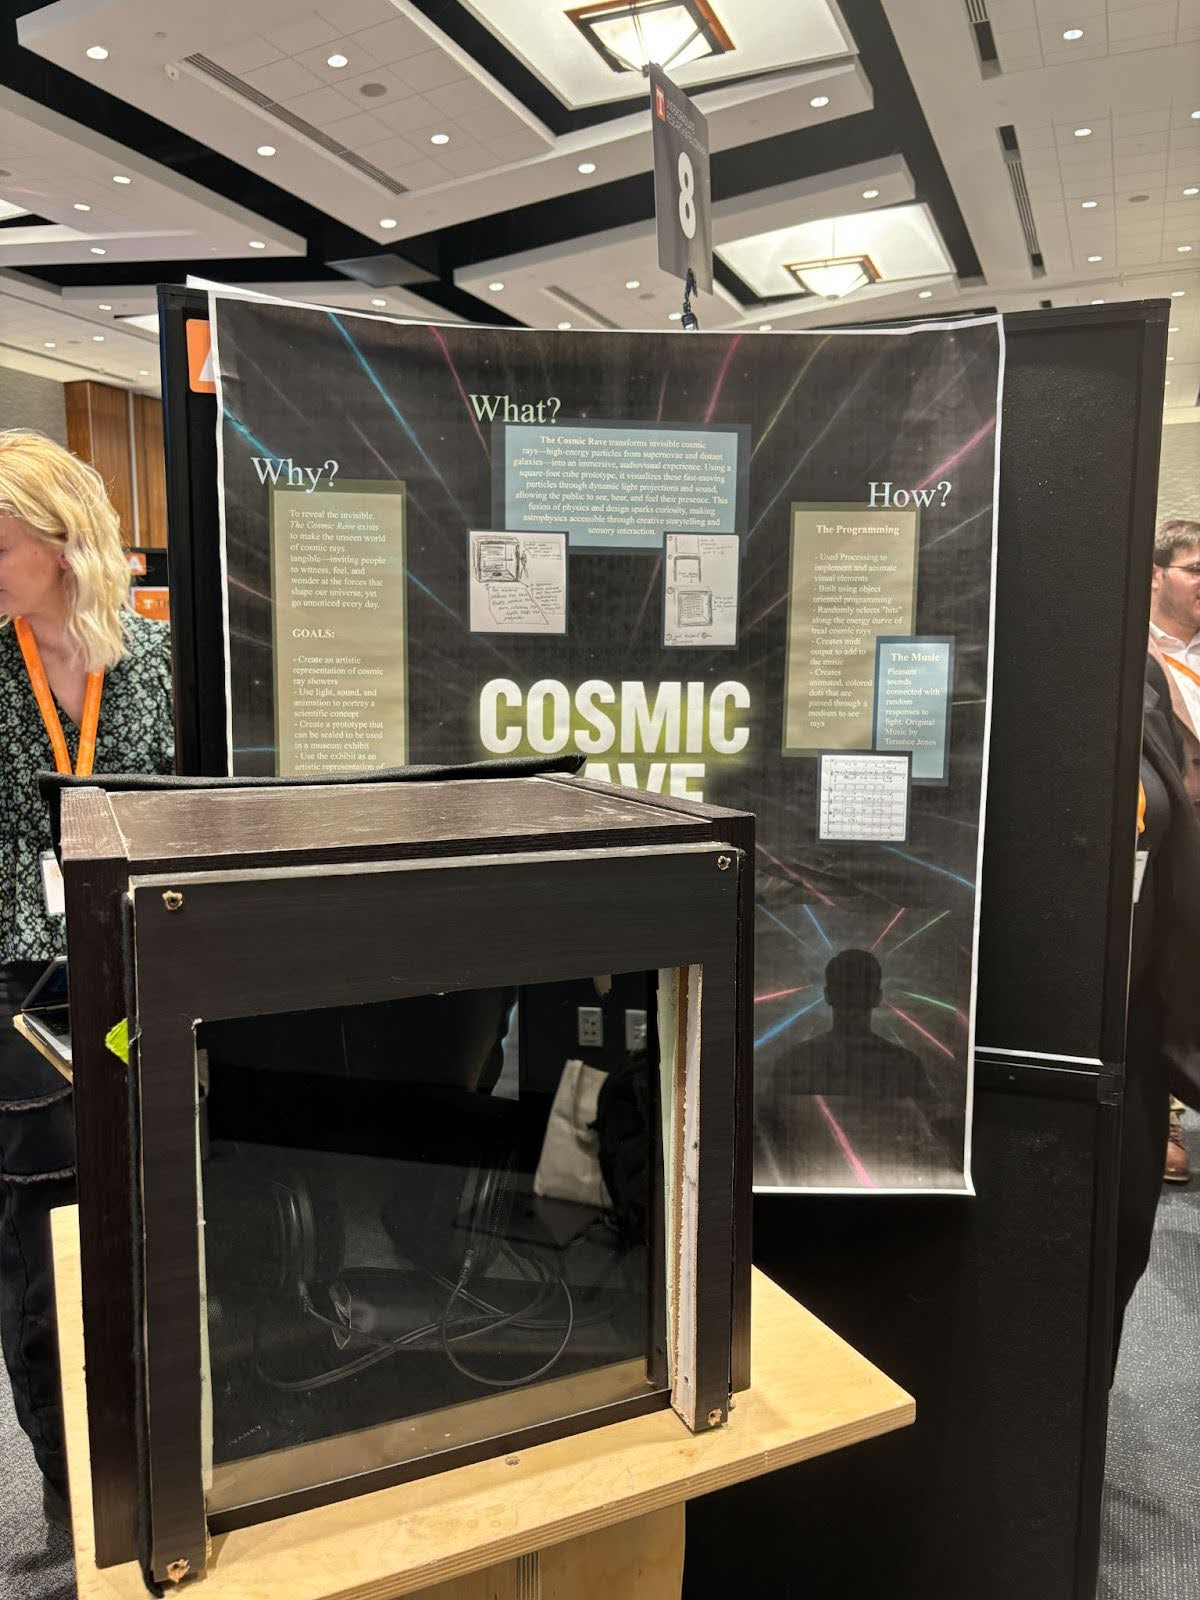
\includegraphics[width=.25\textwidth]{9}
    \caption{Our presentation at EURE\bar{e}A}
\end{center}
\end{wrapfigure}
The final prototype combined light, sound, spatial design, and simple graphics into a unified immersive experience. Our Cosmic Rave installation utilized a projector to project randomly generated light patterns through fog, with the audio elements creating a continuous cosmic pulse. The synchronized MIDI note system offered harmony between the visual and aural components. This created a space where users could "see" and "hear" cosmic rays within a controlled setting.
The plexiglass face, black felt lining, and black wooden box contributed aesthetic value and sonic symbolism, creating a striking visual difference between the multi-colored neon light rays shooting across the box, and the void-like box itself. As intended, the project's modularity provided for scalability. Despite limitations (e.g., we can't 3D print the enclosure), our wood and cardboard prototypes communicated the essence of the cosmic interaction.

\section{Critique of Outcomes}

\textbf{Rose (Must Keep)}
\begin{itemize}
    \item Interdisciplinary fusion of music, design, and physics.
    \item MIDI-synced lighting system tied to the original composition.
    \item Use of fog and light as metaphorical tools to represent the unseen.
    \item Use of dark materials to enhance the quality of the Cosmic Rave.
\end{itemize}




\textbf{Bud (Untested/Unrealized)}
 \begin{itemize}
     \item Scaling the installation to human-size for public exhibition.
     \item Integration of real-time cosmic ray data via sensors or counters.
     \item More refined coding for enhanced light behavior and randomness.
     \item Amount of lighting in the full-scale exhibit (dark enough so the projection is effective, and light enough so people can safely see their way around).
     \item Actuality of rays shooting horizontally without disrupting viewers standing in the space (in the full-scale exhibit).
     \item Use of a speaker as a bench. Would it still be best to go with headphones per individual?
 \end{itemize}


 \textbf{Thorn (Must Leave Out)}
 \begin{itemize}
     \item Over Reliance on DIY materials; compromised visual precision.
    \item Fog machine inconsistencies impacting visual clarity.
    \item Lack of physical interaction from viewers (purely observational).
    \item Improper sealing (too much or too little fog escaping from the cube).
 \end{itemize}


\section{Next Steps}
\textbf{To evolve this prototype into a scalable installation, the following steps are recommended:
}
\\\\
\textbf{Technical:} Look at the code that has been developed. It is left in the git repository listed in the code section. Look at what it does, and change it to fit your needs. Decide on a program to use sound. Midi routing on MacOS is easier than on Linux which is in turn easier than on Windows, but it is possible on any of those systems. 
\\\\
\textbf{Aesthetic:} Determine proper sizing of felt and plexiglass sheet, decide on one shade of black paint, and use a nice quality wood. All of these will help to create a sleek design that does not take away from the experience happening inside the cube. 
\\\\
\textbf{Scalability:} All factors should be mostly straightforward outside of the music element. If the design moves forward with the speaker-bench, the team should determine how to obtain a speaker of proper size, as well as how to enclose it in a way that does not hurt the exhibit, but rather adds to it. 
\\\\
\textbf{Financial:} Apart from initial costs, there shouldn’t be much expense for upkeep other than for the audio element (potentially). Funding can come from, but is not limited to: donations, grants, clients, or pooling together funds. Expenses would include, but not be limited to: wood, fasteners, felt, plexiglass, paint, a projector, a fog machine, a device to run the projector, speakers/headphones, devices to run the audio element, and general upkeep (cleaning of public headphones, etc.)
\\\\	  
\textbf{Feasibility:} Wood, screws/nails/glue, paint, felt and plexiglass should be easily accessible. The audio element may be a bit harder to acquire. With either option (the speaker-bench or headphones) the team must determine how they will acquire a speaker large enough or how they will acquire and store multiple pairs of headphones. With the headphones, the team must also decide on wireless or wired headphones, and determine what the music will be streaming on.

\section{Conclusion}
Our team combined design and science to make the invisible realm of cosmic rays tangible. Using fog, light, music, suitable materials, and metaphor, we produced The Cosmic Rave; an experience that captures how design can render abstract scientific phenomena concrete and memorable. 

To the Fall team: make this idea your own and run. Scale it. Code it. Shine it. Test it on people outside the classroom. Let The Cosmic Rave spread from prototype to phenomenon. The unseen is only invisible because we're not looking for it.
\end{document}
